\documentclass[11pt,twoside,a4paper]{article}
% http://www-h.eng.cam.ac.uk/help/tpl/textprocessing/latex_maths+pix/node6.html symboles de math
% http://fr.wikibooks.org/wiki/Programmation_LaTeX Programmation latex (wikibook)
%=========================== En-Tete =================================
%--- Insertion de paquetages (optionnel) ---
\usepackage[french]{babel}   % pour dire que le texte est en fran{\'e}ais
\usepackage{a4}	             % pour la taille   
\usepackage[T1]{fontenc}     % pour les font postscript
\usepackage{epsfig}          % pour gerer les images
%\usepackage{psfig}
\usepackage{amsmath, amsthm} % tres bon mode mathematique
\usepackage{amsfonts,amssymb}% permet la definition des ensembles
\usepackage{float}           % pour le placement des figure
\usepackage{verbatim}

\usepackage{longtable} % pour les tableaux de plusieurs pages

\usepackage[table]{xcolor} % couleur de fond des cellules de tableaux

\usepackage{lastpage}

\usepackage{multirow}

\usepackage{multicol} % pour {\'e}crire dans certaines zones en colonnes : \begin{multicols}{nb colonnes}...\end{multicols} 

% \usepackage[top=1.5cm, bottom=1.5cm, left=1.5cm, right=1.5cm]{geometry}
% gauche, haut, droite, bas, entete, ente2txt, pied, txt2pied
\usepackage{vmargin}
\setmarginsrb{1.00cm}{1.00cm}{1.00cm}{1.00cm}{15pt}{3pt}{50pt}{20pt}

\usepackage{lscape} % changement orientation page
%\usepackage{frbib} % enlever pour obtenir references en anglais
% --- style de page (pour les en-tete) ---
\pagestyle{empty}

\def\txtTITLE{Cyber Age \& SimulacreS} %%%%% !! TITRE !! %%%%%
\def\imgCORNER{
\includegraphics[width=0.25cm]{../../../../../imgGraphics/logos/glider/logo-glider.png}}

%--- Definitions de nouvelles couleurs ---
\definecolor{verylightgrey}{rgb}{0.8,0.8,0.8}
\definecolor{verylightgray}{gray}{0.80}
\definecolor{lightgrey}{rgb}{0.6,0.6,0.6}
\definecolor{lightgray}{gray}{0.6}

% % % en-tete et pieds de page configurables : fancyhdr.sty

% http://www.trustonme.net/didactels/250.html

% http://ww3.ac-poitiers.fr/math/tex/pratique/entete/entete.htm
% http://www.ctan.org/tex-archive/macros/latex/contrib/fancyhdr/fancyhdr.pdf
\usepackage{fancyhdr}
\pagestyle{fancy}
% \newcommand{\chaptermark}[1]{\markboth{#1}{}}
% \newcommand{\sectionmark}[1]{\markright{\thesection\ #1}}
\fancyhf{}
\fancyhead[LE,RO]{\bfseries\thepage}
\fancyhead[LO]{\bfseries\rightmark}
\fancyhead[RE]{\bfseries\leftmark}
\fancyfoot[LE]{\thepage /\pageref{LastPage} \hfill
	\scriptsize{\txtTITLE} % TITLE
\hfill \imgCORNER }
\fancyfoot[RO]{\imgCORNER \hfill
	\scriptsize{\txtTITLE} % TITLE
\hfill \thepage /\pageref{LastPage}}
\renewcommand{\headrulewidth}{0.5pt}
\renewcommand{\footrulewidth}{0.5pt}
\addtolength{\headheight}{0.5pt}
% \fancypagestyle{plain}{
	% \fancyhead{}
	% \renewcommand{\headrulewidth}{0pt}
% }

\usepackage{lettrine}
\usepackage{fancybox}

\def\imgCORPS{
\includegraphics[width=0.25cm]{../../../../../imgGraphics/rolePlayingGame/SimulacreS/mini12x12/corps.png} }
\def\imgINSTI{
\includegraphics[width=0.25cm]{../../../../../imgGraphics/rolePlayingGame/SimulacreS/mini12x12/instinct.png} }
\def\imgCOEUR{
\includegraphics[width=0.25cm]{../../../../../imgGraphics/rolePlayingGame/SimulacreS/mini12x12/coeur.png} }
\def\imgESPRI{
\includegraphics[width=0.25cm]{../../../../../imgGraphics/rolePlayingGame/SimulacreS/mini12x12/esprit.png} }

\def\imgPERCE{
\includegraphics[width=0.25cm]{../../../../../imgGraphics/rolePlayingGame/SimulacreS/mini12x12/perception.png} }
\def\imgACTIO{
\includegraphics[width=0.25cm]{../../../../../imgGraphics/rolePlayingGame/SimulacreS/mini12x12/action.png} }
\def\imgDESIR{
\includegraphics[width=0.25cm]{../../../../../imgGraphics/rolePlayingGame/SimulacreS/mini12x12/desir.png} }
\def\imgRESIS{
\includegraphics[width=0.25cm]{../../../../../imgGraphics/rolePlayingGame/SimulacreS/mini12x12/resistance.png} }

\def\imgMINER{
\includegraphics[width=0.25cm]{../../../../../imgGraphics/rolePlayingGame/SimulacreS/mini12x12/mineral.png} }
\def\imgVEGET{
\includegraphics[width=0.25cm]{../../../../../imgGraphics/rolePlayingGame/SimulacreS/mini12x12/vegetal.png} }
\def\imgANIMA{
\includegraphics[width=0.25cm]{../../../../../imgGraphics/rolePlayingGame/SimulacreS/mini12x12/animal.png} }
\def\imgHUMAI{
\includegraphics[width=0.25cm]{../../../../../imgGraphics/rolePlayingGame/SimulacreS/mini12x12/humain.png} }
\def\imgMECAN{
\includegraphics[width=0.25cm]{../../../../../imgGraphics/rolePlayingGame/SimulacreS/mini12x12/mecanique.png} }
\def\imgNEANT{
\includegraphics[width=0.25cm]{../../../../../imgGraphics/rolePlayingGame/SimulacreS/mini12x12/neant.png} }

\def\imgPUISS{
\includegraphics[width=0.25cm]{../../../../../imgGraphics/rolePlayingGame/SimulacreS/mini12x12/puissance.png} }
\def\imgRAPID{
\includegraphics[width=0.25cm]{../../../../../imgGraphics/rolePlayingGame/SimulacreS/mini12x12/rapidite.png} }
\def\imgPRECI{
\includegraphics[width=0.25cm]{../../../../../imgGraphics/rolePlayingGame/SimulacreS/mini12x12/precision.png} }

\title{\txtTITLE}
\date{ --- }

%============================= Corps =================================
\begin{document}

\setlength\parindent{0pt} % \noindent for all document

~\\

\vfill

\begin{center}
	\textbf{\Huge \txtTITLE}
\end{center}

\vfill

\tableofcontents

\clearpage

\section{Les Secrets de CyberAge : Les Dactyles}

\begin{multicols}{3}
\scriptsize{
Certaines rumeurs laissent entendre que l'acad{\'e}mie commen\c{c}a sa carri{\`e}re en tant qu'officine de tueurs {\`a} gages ou de terroristes, juste au lendemain de la Grande R{\'e}volution Lib{\'e}rale. C'{\'e}tait alors une secte qui professait l'assassinat politique, et qui tirait ses racines des anarchistes russes de la fin du XIXe si{\`e}cle. L'acad{\'e}mie fut donc au d{\'e}part une sorte d'{\'e}cole d'entra{\^i}nement pour commandos suicide. Mais tr{\`e}s vite, ses membres durent faire face {\`a} la dure concurrence des yakuzas et des tueurs des triades. Son Troisi{\`e}me Secr{\'e}tariat pris alors la d{\'e}cision de quitter la Terre pour les premi{\`e}res {\^I}les de la Lune. {\`A} l'{\'e}poque, c'{\'e}tait une d{\'e}cision tr{\`e}s aventureuse et tr{\`e}s co{\^u}teuse, mais l'acad{\'e}mie avait accumul{\'e} une jolie fortune gr{\^a}ce {\`a} ses assassinats politiques et les {\^I}les {\'e}taient le seul endroit o{\`u} les tueurs yakuzas n'iraient pas les suivre.~\\

Durant pr{\`e}s de quarante ans, on n'entendit plus parler de l'acad{\'e}mie. Les Iles de la Lune {\'e}taient encore un territoire pionnier, beaucoup de stations satellites disparaissaient, se regroupaient ou bien {\'e}taient d{\'e}mantel{\'e}es. Certaines structures d{\'e}riv{\`e}rent en Espace profond sans qu'on prenne la peine de faire des recherches ou d'essayer de sauver les colons qui pouvaient encore s'y trouver. C'{\'e}tait une {\'e}poque sans piti{\'e}. Dans les ann{\'e}es 2060, une rumeur commen\c{c}a {\`a} se r{\'e}pandre dans les services R{\'e}zo des grands TechnoBlocs, on parlait de certains jackeurs, particuli{\`e}rement dou{\'e}s, qui avaient tous un profil identique: ils avaient tous {\'e}t{\'e} form{\'e}s gratuitement dans une acad{\'e}mie des {\^I}les de la Lune. L'acad{\'e}mie Dactyle venait de refaire surface et bien s{\^u}r, personne ne fit le rapport avec la bande de n{\'e}oanarchistes russes qui s'{\'e}taient envol{\'e}s pour les {\'e}toiles quarante ans auparavant, et pourtant...~\\

\textbf{Infos semi-publiques}~\\

\textbf{Extrait d'un rapport sur la secte dites des <<Dactyles>> }~\\

Les Dactyles ont des r{\`e}gles tr{\`e}s strictes et tr{\`e}s {\'e}tranges : aucune ou tr{\`e}s peu de publicit{\'e}, interdiction de prononcer le nom de leurs membres, intervention la plus discr{\`e}te et la plus courte possible. On sait pourtant qu'ils recrutent des jeunes gar\c{c}ons ou filles, les forment {\`a} toutes les techniques du R{\'e}zo, et les renvoient dans la vie normale (sans contrepartie semble-t-il. Une fois ce qu'ils jugent comme {\'e}tant leur t{\^a}che accomplie les Dactyles disparaissent et g{\'e}n{\'e}ralement, le jeune gar\c{c}on ou la jeune fille qui a profit{\'e} de leur g{\'e}n{\'e}rosit{\'e} n'entendra plus jamais parler d'eux. Plusieurs rumeurs affirment qu'ils contr{\^o}lent {\'e}galement en sous main plusieurs {\'e}coles d'enseignement primaire et sup{\'e}rieur, mais aucun network n'a jamais pu en apporter une preuve formelle.~\\

Seules certitudes :
\begin{itemize}
	\item Les Dactyles sont divis{\'e}s en deux coll{\`e}ges non mixtes, la Main Gauche et la Main Droite. 
	\item Leur {\'e}tat major se trouve quelque part sur les {\^I}les de la Lune, ils disposent d'une fortune colossale d'une provenance inconnue et ma{\^i}trisent parfaitement les technologies informatiques.
\end{itemize}

\columnbreak

Comme les francs-ma\c{c}ons, les Dactyles peuvent se reconna{\^i}tre entre eux gr{\^a}ce {\`a} un syst{\`e}me complexe de signes de main et de doigts. Comme  les francs-ma\c{c}ons {\'e}galement, un Dactyle en danger peut esp{\'e}rer le secours de tout autre Dactyle gr{\^a}ce {\`a} un signe de d{\'e}tresse. C'est devenu une plaisanterie dans la Matrice que de rep{\'e}rer des <<signes Dactyles>>. Quand un message est incompr{\'e}hensible, ou qu'il porte une suite de cinq ou dix <<digits>> comme signature, on dit que c'est un message Dactyle.~\\

Ainsi le dicton : <<Les doigts de ta main droite sont tes Dactyles, et ceux de ta main gauche doivent {\^e}tre abandonn{\'e}s aux sorci{\`e}res>> semble ne rien vouloir dire. Bien entendu on a tout dit sur eux : qu'ils {\'e}taient des extraterrestres, des agents des Sept Dragons, des cyborgs... Mais personne aujourd'hui n'est encore capable de dire quels sont les buts de l'acad{\'e}mie Dactyles. Reste que la majorit{\'e} des grands jackeurs est issue de leurs rangs depuis pr{\`e}s de vingt ans.~\\

\textbf{Archiv{\'e} au CTI -- \texttt{MediASsisT} }~\\

\textbf{Mythologie}

Si l'on recherche dans les bases de donn{\'e}es au mot Dactyles on ne trouvera que des r{\'e}f{\'e}rences mythologiques, ce qui est un peu frustrant pour le pirate moderne.                                  
Les cinq Dactyles m{\^a}les {\'e}taient des forgerons, les cinq Dactyles femelles {\'e}taient des magiciennes. Leur origine est obscure. Il semblerait que Rh{\'e}a enceinte de Zeus, enfon\c{c}a ses doigts dans le sol pour soulager ses douleurs, et ainsi naquirent les Dactyles.~\\

Les Dactyles de la main droite sont des forgerons et des magiciens. ils travaillent le fer, et le fer fut dans l'antiquit{\'e} un m{\'e}tal sacr{\'e}. D'origine m{\'e}t{\'e}orique, {\`a} forte teneur en nickel, il ne rouillait presque jamais, c'est avec lui qu'on fabriquait les meilleures armes, il {\'e}tait bien entendu tr{\`e}s rare et la d{\'e}couverte d'une m{\'e}t{\'e}orite charg{\'e}e en fer {\'e}tait consid{\'e}r{\'e}e comme un pr{\'e}sent des dieux.~\\

Ce sont les Dactyles femmes qui enseign{\`e}rent les Myst{\`e}res de la Triple D{\'e}esse {\`a} Orph{\'e}e. On n'en sait pas plus.~\\

\textbf{Infos secr{\`e}tes}

La Main Gauche des Dactyles, qui se charge de l'enseignement des techniques de l'informatique est compos{\'e}e uniquement de femmes. Il n'y a pas de lieu propre {\`a} l'enseignement. Les <<sorci{\`e}res>>, comme elles se nomment parfois elles-m{\^e}mes, donnent des le\c{c}ons particuli{\`e}res ou montent des cours pour un temps donn{\'e}.~\\

Mais bien peu de gens connaissent l'autre face de l'acad{\'e}mie, il s'agit de l'activit{\'e} de la Main Droite ou la <<main masculine des Dactyles>>. En moins de cinquante ans elle s'est hiss{\'e} de fa\c{c}on tout {\`a} fait occulte au tout premier rang des fabricants d'armes l{\'e}g{\`e}res. Les ateliers secrets de l'acad{\'e}mie sont {\`a} l'heure actuelle capable de produire les meilleures armes l{\'e}g{\`e}res du monde et ce sans que le nom de l'acad{\'e}mie n'apparaisse une seule fois dans les rapports d'experts sur la production militaire mondiale.~\\

\columnbreak

Les armuriers de l'acad{\'e}mie vendent discr{\`e}tement leur production gr{\^a}ce {\`a} des interm{\'e}diaires et {\`a} des pr{\^e}tes noms. D'ordinaire ils vendent {\`a} tout le monde mais certaines commandes ne sont pas honor{\'e}es, les armuriers ne s'en expliquent jamais, si le client insiste, un contrat yakuza le ram{\`e}ne assez vite {\`a} la raison.~\\
 
Les armuriers de l'acad{\'e}mie ne font pas que fabriquer des armes, ils en inventent aussi, ils sont m{\^e}me {\`a} la pointe de la recherche dans plusieurs domaines, laser, armes molles, identification de cibles. Ils sont {\'e}galement tr{\`e}s sp{\'e}cialis{\'e}s dans les programmes d'attaques et de d{\'e}fense en cyberspace, notamment sur les mod{\`e}les de Glace de troisi{\`e}me g{\'e}n{\'e}ration, un type de Glace totalement reg{\'e}n{\'e}rable et virtuellement impossible {\`a} percer.~\\
 
Bien s{\^u}r, si on savait d'o{\`u} venaient les derni{\`e}res g{\'e}n{\'e}rations de Glace et de programmes tueurs depuis pr{\`e}s de dix ans, toutes les acad{\'e}mies seraient imm{\'e}diatement prise d'assaut par les forces des TechnoBlocs li{\'e}s {\`a} la vente d'armes, dans cette perspective on comprend mieux la discr{\'e}tion des secr{\'e}taires de l'acad{\'e}mie.~\\
 
Si on pouvait demander {\`a} un responsable de l'armurerie de l'Acad{\'e}mie la raison pour que cette derni{\`e}re ne fabrique que des armes l{\'e}g{\`e}res il aurait pourrait r{\'e}pondre quelque chose dans le genre <<Justement pour qu'on ne se serve que le moins possible des armes lourdes>>. Bien entendu les {\'e}normes profits de la Main Droite servent {\`a} financer les non moins {\'e}normes pertes de la Main Gauche.~\\

\textbf{Donn{\'e}es techniques}~\\

Les Dactyles sont environ une centaine (60 \% de femmes), dont la moiti{\'e} vit sur une base spatiale aux environs des lunes de Jupiter. Leur base proche est sur une des {\^I}les de la Lune. Ils poss{\`e}dent (sur Jupiter) un I.A.Q. de valeur 80, nomm{\'e}e Rh{\'e}a, sp{\'e}cialis{\'e}e dans la cr{\'e}ation de logiciels (Glaces et autres). Ce sont les Dactyles qui fournissent 60 \% des Glaces du R{\'e}zo, notamment les Glaces noires (60 \%).~\\

\textbf{Talents typiques d'une Dactyle} : Piratage +2, Informatique +2, Pratiques shamanique ou M{\'e}ditation zen +2, Enseignement +1, Com{\'e}die +1. Presque jamais de c{\^a}blage, sauf c{\^a}blage Matrice sp{\'e}cial (suivi d'une th{\'e}rapie pour remonter l'{\'E}quilibre psychique perdu).~\\

\textbf{Talents typiques d'un Dactyle} : Ing{\'e}nierie des armes +1, Armes l{\'e}g{\`e}res +1 ou 0, Commerce +1, Biologie/g{\'e}n{\'e}tique +1. En g{\'e}n{\'e}ral ils ont des c{\^a}blages divers interfac{\'e}s {\`a} des armes sp{\'e}ciales. 

\begin{center} \rule{4cm}{0.5mm} \end{center}

\texttt{\scriptsize{(Originellement Publi{\'e} dans : Casus Belli Hors s{\'e}rie n 16, Auteur : Pierre Rosenthal)}}

} % end scriptsize
\end{multicols} 

\clearpage

\section{CyberAge, CyberEspace et Matrice : La Plong{\'e}e}
%% Univers Pour : 
\includegraphics[width=3cm]{../../../../../imgGraphics/rolePlayingGame/SimulacreS/logos/logoSimulacreS01.png}~\\

\begin{minipage}[ht]{0.45\textwidth}
% \textbf{\Large La plong{\'e}e}~\\
\textbf{\scriptsize Le R{\'e}zo, la Matrice, le cyberspace, tous ces mots d{\'e}signent la m{\^e}me chose tout en n'en montrant qu'une partie. Et quand des millions de connect{\'e}s partagent un m{\^e}me espace en croyant sinc{\`e}rement qu'il y a "quelque chose" derri{\`e}re tout \c{c}a, il est naturel -- alors que la technologie permet de manipuler les r{\^e}ves -- que ceux-ci se concr{\'e}tisent. }~\\

\texttt{\scriptsize{(Originellement Publi{\'e} dans : Casus Belli Hors s{\'e}rie n 16, Auteur : Pierre Rosenthal)}}
\end{minipage} \hfill \begin{minipage}[ht]{0.45\textwidth}
\colorbox{lightgrey}{ \shadowbox{\scriptsize %
\begin{minipage}[ht]{0.90\textwidth}
\textbf{Glace Noire}~\\
Certaines Glaces peuvent d'un seul coup faire basculer un esprit dans le Kernel. Autant dire que pour quelqu'un de non pr{\'e}par{\'e}, c'est le choc traumatique assur{\'e}, d'o{\`u} les << l{\'e}gendes >> de jackeurs qui ont << br{\^u}l{\'e} >> leur cerveau.~\\
\textbf{Math{\'e}matiques chaotiques}~\\
Certains math{\'e}maticiens de tr{\`e}s haut niveau arrivent {\`a} aller dans le Kernel en utilisant le talent Math{\'e}matiques chaotiques {\`a} la place de celui de M{\'e}ditation Zen. Les diff{\'e}rences sont: pas de possibilit{\'e} de passer dans la Jungle; et le test de souvenir se fait sans le malus de -4 d{\`e}s que l'on veut des donn{\'e}es qui peuvent s'exprimer en mots ou en chiffres (pas plus de l'{\'e}quivalent d'une page de livre).~\\
\end{minipage} } }%
\end{minipage}

\begin{multicols}{3}
\scriptsize{

\textbf{\Large La Jungle}~\\

Dans l'encyclop{\'e}die, on vous a dit qu'il existait deux niveaux pour visiter le R{\'e}zo : HyperNet et la Matrice. En fait, il existe encore deux autres niveaux que peu de jackeurs connaissent, m{\^e}me si les termes qui les d{\'e}finissent leur sont familiers.~\\

Tout d'abord, au niveau inf{\'e}rieur {\`a} la Matrice, il y a un niveau que nous d{\'e}signerons sous le nom de Jungle (parfois connu sous le nom de Grand Bleu -- d'o{\`u} le terme de plong{\'e}e, ou Reptilien, ou Jurassique). Ce niveau correspond {\`a} celui que nous appelons dans nos ordinateurs actuels : syst{\`e}me d'exploitation. Dans les ann{\'e}es 2080, on ne programme quasiment plus en code. On donne des instructions symboliques. Et les syst{\`e}mes communiquent entre eux par des techniques d'HDI (Holographic Dreams Image, IRH en fran\c{c}ais). Ces flots d'HDI sont des donn{\'e}es extr{\^e}mement compactes -- cod{\'e}es comme des images fractales, de m{\^e}me type que celles produites par les machines {\`a} r{\^e}ves. Ils permettent de faire circuler en m{\^e}me temps des donn{\'e}es, des instructions et des configurations (nouvelle fa\c{c}on d'appr{\'e}hender les donn{\'e}es). Au XXI' si{\`e}cle (en faisant un raccourci), on peut dire que les ordinateurs communiquent entre eux en r{\^e}vant, ou en s'{\'e}changeant des r{\^e}ves.~\\

\textbf{\large Ce qui se passe dans la Jungle}~\\

Dans la Jungle, fe jackeur se verra comme il s'imagine en r{\^e}ve. Il n'y aura plus de Glaces, de TechnoBlocs, de zones de donn{\'e}es. Si le jackeur s'imagine comme un chevalier, il sera recouvert d'une armure brillante, chevauchant peut-{\^e}tre dans une verte plaine. Tant que le jackeur navigue dans des zones visit{\'e}es par tout le monde, c'est sa vision qui s'impose. Quand il approche d'un TechnoBloc, c'est l'image inconsciente de la structure qui s'impose. En g{\'e}n{\'e}ral on rencontrera un gigantesque robot, un comptable retors, etc. Mais il faut bien dire que nombre de TechnoBlocs se voient comme de redoutables pr{\'e}dateurs, et les Sept Dragons n'ont pas vol{\'e} leur nom.~\\

Si on veut << voler >> une donn{\'e}e au TechnoBloc, il faudra le vaincre. Ce qui peut {\^e}tre tr{\`e}s dangereux. On peut aussi, ce qui est impossible dans la Matrice, dialoguer avec le syst{\`e}me d'un TechnoBloc, le persuader, le charmer, lui demander des renseignements. Et peut-{\^e}tre r{\'e}ussir. Une fois sorti de la Jungle, dans la Matrice, on retrouvera les informations donn{\'e}es ou vol{\'e}es dans sa m{\'e}moire informatique comme si on venait de les pirater.~\\

\textbf{\Large Le Kernel}~\\

Une Intelligence Artificielle est une cr{\'e}ature du R{\'e}zo, et aucun humain ne peut penser un jour l'{\'e}galer en habilit{\'e} et en vitesse (une I.A. fait cent mille millions de milliards de fois plus d'op{\'e}rations simultan{\'e}es qu'un humain). Mais c'{\'e}tait compter sans l'astuce et la philosophie de certains moines jackeurs tib{\'e}tains, qui d{\'e}velopp{\`e}rent la technique de << plong{\'e}e profonde >>, dite << petit nirvana >>. Puisque les ordinateurs communiquent par une certaine forme de pens{\'e}e, il suffisait de rendre son esprit proche de ce m{\^e}me mode, devenir un relais, une m{\'e}moire pour le R{\'e}zo, dispara{\^i}tre pour se fondre dans la Matrice. Il ne reste alors plus qu'{\`a} << d{\'e}river >> dans le Kernel (le niveau inf{\'e}rieur {\`a} la Jungle, celui o{\`u} les flots HDI naviguent de fa\c{c}on r{\'e}flexe, sans plus aucune volont{\'e} consciente) jusqu'aux abords du lieu que l'on veut conna{\^i}tre. Le syst{\`e}me informatique utilisera alors le cerveau du jackeur comme relais, s'appropriant ses synapses. Une fois la transe termin{\'e}e, le jackeur n'a alors plus qu'{\`a} se << souvenir >>, les donn{\'e}es qu'il cherche sont quelque part dans sa m{\'e}moire.~\\

\textbf{\large Les dangers du Kernel}~\\

Le probl{\`e}me d'ouvrir son cerveau aux ordinateurs est que l'on ouvre la porte {\`a} toutes les manipulations. Tout d'abord, si son esprit n'est pas assez vide (il ne faut plus penser {\`a} rien qu'a objectif) les logiciels sentent une r{\'e}sistance et br{\^u}lent litt{\'e}ralement le cerveau. Ensuite il faut savoir verrouiller des parties de son cerveau, sinon on se r{\'e}veille en ayant perdu toute sa m{\'e}moire, et parfois pire encore (se souvenir que 3 plus 18 font 1, et que la soude caustique se d{\'e}guste {\`a} temp{\'e}rature ambiante, est assez handicapant). Enfin, il faut arriver {\`a} se souvenir de donn{\'e}es qui auront peut-{\^e}tre {\'e}t{\'e} rang{\'e}e tr{\`e}s loin dans sa m{\'e}moire. Il n'est pas rare qu'un jackeur tib{\'e}tain de 60 ans, apr{\`e}s une visite au Kernel, se "souvienne" avoir inscrit un code sur un papier quand il avait 12 ans. Mais ce code {\'e}tait-il C2A4S6 ou C3A46S ? Le souvenir remonte quand m{\^e}me {\`a} 48 ans dans le pass{\'e} pour le moine.~\\

\textbf{\Large En jeu}~\\

\textbf{\large Entrer dans la Jungle/Kernel}~\\

Il faut d'abord {\^e}tre dans la Matrice. Puis faire un test de mise en transe. Un jackeur qui ne sait pas que la Jungle et le Kernel existent n'aura pas cette id{\'e}e de lui m{\^e}me. Le test vaut Esprit~\imgESPRI + D{\'e}sir~\imgDESIR + Humain~\imgHUMAI + [M{\'e}ditation Zen] -4. La M{\'e}ditation Zen est un talent qui est une technique sp{\'e}cialis{\'e}e avec une base de -4. Si le test {\'e}choue, on subit une d{\'e}connexion brutale (perte de 3PS). Si on r{\'e}ussit, la Marge de R{\'e}ussite indique jusqu'o{\`u} on peut descendre.~\\
\textbf{Marge de 1 {\`a} 3} : on reste {\`a} la frange, sans pouvoir descendre dans la Jungle.~\\
\textbf{Marge de 4 {\`a} 16} : Jungle. ~\\
\textbf{Marge de 17 {\`a} 20} : on est entre Jungle et Kernel, cela permet {\`a} ceux qui ne connaissent que la Jungle de savoir qu'il y a quelque chose dessous.~\\
\textbf{Marge de 21 et plus} : Kernel.~\\

\textbf{\large {\^E}tre et agir dans la Jungle}~\\

Agir dans la Jungle est tout simplement jouer {\`a} un jeu de r{\^o}le dans le jeu de r{\^o}le. C'est au meneur de jeu de trouver des adversaires, des pi{\`e}ges, des qu{\^e}tes {\`a} accomplir pour avoir les renseignements. Tous les talents sont conserv{\'e}s par le personnage en Jungle. II n'a plus d'{\'e}quipement autre que le mat{\'e}riel standard correspondant {\`a} l'univers o{\`u} il {\'e}volue. On {\'e}change ses valeurs de Corps et Instincts pour tous les tests qu'il a {\`a} faire. De plus un malus affecte tous ses tests d{\`e}s qu'il va << loin >> (sur une autre grille, une autre SatZone). Un personnage qui perd tous ses PS ou tous ses PV est {\'e}ject{\'e} de la Jungle. Quand on perd des PV, ils sont convertis en EP {\`a} la sortie de la Jungle. Pour sortir volontairement de la Jungle, il faut r{\'e}ussir un test Esprit~\imgESPRI + Action~\imgACTIO + Humain~\imgHUMAI + [M{\'e}ditation Zen]. En cas d'{\'e}chec, il y a d{\'e}connexion brutale.~\\

\textbf{\large {\^E}tre et agir dans le Kernel}~\\

Dans le Kernel il faut d'abord ne pas {\^e}tre, donc r{\'e}ussir un test Esprit~\imgESPRI + R{\'e}sistance~\imgRESIS + N{\'e}ant~\imgNEANT + [M{\'e}ditation Zen] (le N{\'e}ant vaut -1). En cas d'{\'e}chec, on subit [B] EP et on est d{\'e}connect{\'e}. Ensuite il faut se laisser d{\'e}river dans le Kernel jusqu'{\`a} son objectif, test Esprit~\imgESPRI + D{\'e}sir~\imgDESIR + M{\'e}canique~\imgMECAN + [M{\'e}ditation Zen]. Si on {\'e}choue, un programme passe dans une partie du cerveau et le br{\^u}le, faisant [B]PV de d{\'e}g{\^a}ts d{\'e}finitifs sur une partie du corps. Il faut ensuite savoir quand remonter, et faire un test Esprit~\imgESPRI + Perception~\imgPERCE + M{\'e}canique~\imgMECAN + [M{\'e}ditation Zen]. Si ce test {\'e}choue, aucune autre cons{\'e}quence que celle de ne pas avoir r{\'e}ussi. Enfin, il faut se souvenir de ce que l'on a {\'e}t{\'e} chercher, avec un test Esprit~\imgESPRI + Action~\imgACTIO + Humain~\imgHUMAI + [M{\'e}ditation Zen] -4. Si le test {\'e}choue, on n'aura que des souvenirs fragmentaires. Le gros avantage du Kernel est que l'on n'y rencontre plus ni Glace ni I.A. Le gros d{\'e}faut : on met son cerveau en gage {\`a} chaque fois.~\\

} % end scriptsize
\end{multicols} 

\clearpage

\section{Annabella Grubert, cyber psychiatre}

\textbf{\textit{\small Dans l'univers impitoyable CyberPunk, les jackeurs (pirates ou inconscients d{\'e}r{\'e}gulateurs du syst{\`e}me) mettent leur cerveau en jeu pour aller chercher le saint graal du futur -- l'information. Malheureusement nombreux sont ceux qui se grillent les neurones au contact des glaces noires noires. Une fois la passe destructrice effectu{\'e}e, sont-ils vraiment irr{\'e}cup{\'e}rables ?}}~\\
\texttt{\scriptsize{(\textbf{Le petit capharna{\"u}m} n 22 --- Texte : \textbf{Pierre Rosenthal} / Illustration : \textbf{{\'E}ric Puech)} }}

\begin{multicols}{2}
\footnotesize{

\textbf{\Large Refus d'existence}~\\

Que les pirates informatiques existent, personne n'en disconvient. Qu'ils s'appellent jackeurs, deckers, runners, cowboys, \c{c}a aussi tout le monde le sait. Mais que les TechnoBlocs (et autres m{\'e}gacorps) utilisent sciemment des programmes de d{\'e}fense qui bousillent le cerveau des intrus, c'est plus discutable. Non pas que ce soit un secret, mais c'est plut{\^o}t un fait indiscut{\'e} pour lequel il n'y a pas vraiment de preuves. Apr{\`e}s tout, ceux qui ont rencontr{\'e} une glace noire sont rarement en {\'e}tat d'en parler.~\\

\textbf{\Large L'Institut du Bon Secours}~\\

Que faire alors de ces l{\'e}gumes vivants, surtout s'ils n'ont pas pay{\'e} leurs cotisations sociales. Annabella Grubert a trouv{\'e} une solution. Ag{\'e}e d'une trentaine d'ann{\'e}es, cette ancienne missionnaire dans les Zones Blanches d'Afrique centrale a ouvert {\`a} Paris un hospice pour les d{\'e}ficients mentaux.~\\

La vocation du Bon Secours est de porter assistance aux d{\'e}biles, aux malform{\'e}s c{\'e}r{\'e}braux (mutants, malades) et {\`a} quelques junkies au cerveau rong{\'e} par la drogue. Ayant parmi ses anciens amis des jackeurs au cerveau grill{\'e}, elle a tent{\'e} de les faire entrer comme patients. Devant le refus de l'administration de reconna{\^i}tre ces cas, elle utilise d{\'e}sormais une m{\'e}thode peu chr{\'e}tienne pour les faire admettre. Elle leur fait absorber suffisamment de drogue pour qu'ils passent les tests d'entr{\'e}e>> de l'institut. Elle esp{\`e}re les sevrer apr{\`e}s, si elle arrive {\`a} les r{\'e}parer.~\\

\textbf{\Large Doctoresse Jekyll}~\\

Les patients de l'institut qui nous int{\'e}ressent se classent en deux cat{\'e}gories. La premi{\`e}re, ce sont les arpenteurs de la Matrice classique qui ont rencontr{\'e} une glace noire (celle-ci leur a vraiment bouff{\'e} des neurones). Pour les soigner, il faut leur r{\'e}parer physiquement le cerveau. La deuxi{\`e}me cat{\'e}gorie concerne ceux qui se sont immerg{\'e}s trop profond{\'e}ment dans les niveaux Jungle ou Kernel (voir Cyber Age p. 85) de la Matrice et n'en sont jamais remont{\'e}s.~\\

Pour soigner ces patients, Annabella Grubert a d{\'e}velopp{\'e} une m{\'e}thode psychiatrique "de l'int{\'e}rieur ". Elle se connecte sur un r{\'e}seau local, en lien direct avec le cerveau du malade, et va discuter avec toutes les strates conscientes et inconscientes du sujet. La m{\'e}thode est relativement efficace avec les patients de la seconde cat{\'e}gorie. Elle les retrouve g{\'e}n{\'e}ralement prostr{\'e}s dans un univers fantasmatique plut{\^o}t sombre (o{\`u} si{\`e}gent parfois des cauchemars) et elle entreprend de les rassurer. Dans cette Matrice, elle prend souvent l'apparence d'une religieuse rayonnante, calme et charismatique, tr{\`e}s proche de ce qu'elle est dans la r{\'e}alit{\'e}. Il est courant que ses anciens patients l'appellent par la suite la Dame du Bon Secours, et lui vouent une grande admiration.~\\

Pour les sujets dont le cerveau est vraiment endommag{\'e}, elle proc{\`e}de en rajoutant des faux souvenirs, des d{\'e}rivations mentales. Son but: faire oublier l'{\'e}pisode traumatisant d{\`e}s qu'il revient {\`a} la conscience. En g{\'e}n{\'e}ral, le patient gu{\'e}ri se "rappellera" qu'il se droguait (m{\^e}me si c'est faux) et que, apr{\`e}s de nombreuses pertes de conscience, il a d{\'e}cid{\'e} de se faire d{\'e}sintoxiquer {\`a} l'institut du Bon Secours, o{\`u} soeur Annabella lui a prodigu{\'e} soutien et affection.~\\

\textbf{\Large Sister Hyde}~\\

Les subventions sont rares {\`a} l'institut (les TechnoBlocs ne sont pas pr{\^e}ts {\`a} payer pour les non-productifs), et le Bon Secours re\c{c}oit peu de dons (soeur Annabella se m{\'e}fie des m{\'e}dias). Mais la religieuse a trouv{\'e} un moyen tr{\`e}s lucratif de rentabiliser ses gu{\'e}risons, et de participer {\`a} la " grande r{\'e}volution contre les TechnoBlocs d{\'e}shumanisants". Elle a remarqu{\'e} que la structure d'un cerveau grill{\'e} avait souvent un rapport avec le type de glace rencontr{\'e}. Gr{\^a}ce {\`a} la divine Providence, une grande puissance de d{\'e}duction et une pointe de g{\'e}nie, elle arrive {\`a} d{\'e}crypter ces blessures et {\`a} identifier la glace responsable du dommage, et par l{\`a} de concevoir des BriseGlaces adapt{\'e}s {\`a} ces protections. Ce dont elle ne se prive pas.~\\

Quant aux autres patients, ceux qu'elle a remont{\'e}s du fin fond de leur inconscient, elle a remarqu{\'e} qu'elle pouvait aider grandement leur m{\'e}moire en allant directement faire le m{\'e}nage dedans, en {\'e}liminant les parasites. Ces plongeurs en Matrice profonde viennent donc souvent la voir apr{\`e}s des passes diff iciles, pour se faire aider {\`a} retrouver les donn{\'e}es enfouies dans leur cerveau. Donn{\'e}es qu'ils offrent alors {\'e}galement {\`a} l'institut du Bon Secours.~\\

Annabella Grubert est-elle aussi d{\'e}sint{\'e}ress{\'e}e qu'il y parait ? Est-elle une id{\'e}aliste r{\'e}volutionnaire, un agent des Dactyles? Si les Technoblocs apprenaient sa m{\'e}thode, ne 1'utiliseraient-ils pas eux-m{\^e}mes en sacrifiant de pauvres jackeurs kamikazes ? Faut-il la d{\'e}noncer, la laisser vivre, lui pr{\^e}ter assistance ? Et si un jour vous jouiez un jackeur et que vous soyez soign{\'e} par elle ?~\\

\textbf{\large \emph{Caract{\'e}ristique pour Simulacres/Cyber Age}}~\\

\textbf{\large Annabella Grubert}~\\

\textbf{PMJ} : Exceptionnel~\\
\textbf{M{\'e}tier} : Missionaire/Psychiatre/Jackeuse~\\
\textbf{Talents} : M{\'e}ditation transcendantale+3, Piratage +2, Psychiatrie+2, Informatique +1, Psychologie +1, Survie en milieu contamin{\'e} +1, M{\'e}decine 0, survie en milieu tropical 0.~\\
Elle n'a aucun {\'e}quipement cybern{\'e}tique, et ne se connecte que par des {\'e}lectrodes.~\\

} % end footnotesize
\end{multicols} 

\clearpage

\section{Aide de jeu CyberAge/SangDragon}

\textbf{\textit{\small Notre hors-s{\'e}rie \emph{CyberAge}, jeu de r{\^o}le cyberpunk, est toujours disponible. Voici quelques suggestions de sc{\'e}narios plut{\^o}t classiques {\`a} d{\'e}velopper si vous {\^e}tes en manque d'id{\'e}es. En ce qui concerne SangDragon, jeu de r{\^o}le m{\'e}di{\'e}val-fantastique, nous vous proposons un syst{\`e}me alternatif pour les composants de sort (dont l'usage sera imm{\'e}diat avec L'entrep{\^o}t de Ma{\^i}tre Sorbier, une aide de jeu de l'Encyclop{\'e}die m{\'e}di{\'e}vale-fantastique volume II, hors-s{\'e}rie n 17). }}~\\

\texttt{\scriptsize{(Source : \textbf{Petit Capharna{\"u}m} n 19, texte : \textbf{Pierre ROSENTHAL} et \textbf{Jean-Pierre P{\'E}CAU}, illustration : \textbf{{\'E}ric PUECH)} }}~\\

\begin{multicols*}{3}
\footnotesize{

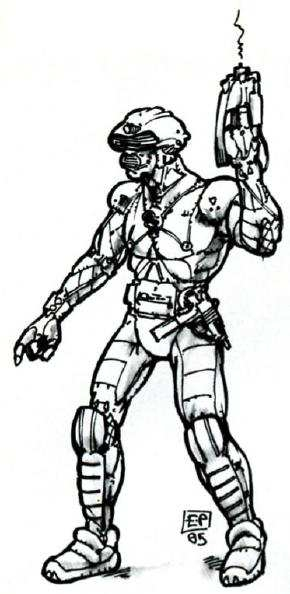
\includegraphics[width=0.30\textwidth]{img/persoRunnerGun.jpg}

\textbf{\textit{Pour CyberAge}}~\\

\texttt{Trois mini sc{\'e}narios}~\\

\textbf{Vengeance maya}~\\

Les personnages prennent le frais dans leur bar habituel, le Gentleman's Looser, quand un homme entre et d{\'e}sint{\`e}gre Pat Desnos, le patron et ami des PJ. Le tueur semble en transe et invuln{\'e}rable aux tirs de riposte des consommateurs, bien qu'il ne porte apparemment pas de gilet pareballes. Il est en effet enti{\`e}rement recouvert d'une armure nano qui le met {\`a} l'abri des tirs d'armes l{\'e}g{\`e}res. Il est {\'e}quip{\'e} d'un laser haute puissance avec deux charges seulement (il en a utilis{\'e} une) et d'un mini pistolet-mitrailleur au c{\^o}t{\'e}.~\\

Torr{\`e}s, l'homme en question, n'en est pas {\`a} son cou d'essai et ne frappe pas au hasard. Pat Desnos, sa septi{\`e}me victime, et tous les autres, {\'e}taient d'anciens Mercs qui avaient servi dans la m{\^e}me unit{\'e} lors des Guerres am{\'e}ricaines contre les rebelles mayas. Durant une op{\'e}ration, Torr{\`e}s fut s{\'e}rieusement bless{\'e}. Il a toujours pens{\'e} que ses camarades l'avaient abandonn{\'e} et depuis, il m{\^u}rit des projets de vengeance.~\\
Les personnages enqu{\^e}tent sur la mort de leur ami et l'identit{\'e} de son assassin.~\\

Profitez-en pour les lancer sur autant de fausses pistes que vous le d{\'e}sirez (racket des yakuzas, vieux ennemis, etc.) afin de cultiver la parano{\"i}a des joueurs. La v{\'e}rit{\'e} appara{\^i}t quand la fille de Desnos leur montre un vieil holo repr{\'e}sentant le squad de son p{\`e}re. On y reconna{\^i}t non seulement Torr{\`e}s, mais {\'e}galement toutes ses derni{\`e}res victimes. Trois hommes sont encore en vie, dont un riche repr{\'e}sentant d'un TechnoBloc de la c{\^o}te m{\'e}diterran{\'e}enne, le seul Merc ayant r{\'e}ussi socialement. Les personnages vont aller le trouver pour le mettre en garde. Ulysse Papandr{\'e}ous est un dur {\`a} cuire, et m{\^e}me s'il accepte d'engager les personnages, il ne fera rien pour {\'e}viter la confrontation avec Torr{\`e}s.~\\

Un des personnages finit par {\^e}tre captur{\'e} par Torr{\`e}s, qui le drogue et lui ordonne de ramener les autres dans son repaire pour s'en d{\'e}barrasser. Les PJ peuvent tomber ou non dans le pi{\`e}ge. Dans tous le cas, ils doivent retrouver Torr{\`e}s avant qu'il ne mette sa vengeance {\`a} ex{\'e}cution.~\\

\textbf{Zone de feu}~\\

Un des personnages aide Slide, un de ses amis d'enfance. Slide est un Sauvage urbain dont le clan est parvenu {\`a} f{\'e}d{\'e}rer plusieurs bandes d'une zone et arr{\^e}ter du coup la guerre qu'elles se livrent. Le personnage est attir{\'e} dans un hangar, drogu{\'e} par un Wampire, puis remis {\`a} un << Obeyin >>, un chef de clan yakuza qui ne voit pas d'un tr{\`e}s bon oeil l'entente cordiale qui se dessine dans sa zone d'influence (les ventes d'armes vont b{\^e}tement baisser).~\\

Asuma Korino, le yakuza, drogue le personnage pour le dresser {\`a} tuer Slide, le conditionnement est plus ou moins long selon la r{\'e}sistance du personnage. Pendant ce temps, on peut esp{\'e}rer que ses camarades finissent par retrouver le lieu de son enl{\`e}vement : des SDF l'ont vu entrer dans le hangar et jamais ressortir.~\\

Le reste du sc{\'e}nario est une course de vitesse entre le personnage conditionn{\'e} et les autres, puis le retour dans le labo des yakuzas pour y faire le m{\'e}nage.~\\

Bien entendu, la mort de Slide rallumerait la guerre des clans, et les personnages se retrouveraient pris entre deux feux, d{\'e}sign{\'e}s par tous comme les assassins de la paix.~\\

\textbf{La nuit des hologrammes}~\\

MediASsist se voit confier une mission : assurer la protection d'un juge ind{\'e}pendant de la ville de Paris.~\\

Plusieurs de ses coll{\`e}gues sont d{\'e}j{\`a} morts dans des conditions myst{\'e}rieuses, tous avaient re\c{c}u auparavant un petit cercueil en bois noir. Le juge assiste {\`a} un holo spectacle, quand un des hologrammes l'attaque et tente de le tuer. Les personnages interviennent et d{\'e}branchent rapidement le mat{\'e}riel. Ils ne savent quoi penser : c'est la premi{\`e}re fois qu'il est question d'une tentative d'assassinat via hologramme, qui par d{\'e}finition n'est qu'une source lumineuse inoffensive.~\\

En observant avec attention les bandes holo, les personnages parviennent {\`a} isoler une marque de fabrique, un petit {\'e}tablissement sur les quais de la Seine. Lorsqu'ils s'y rendent, ils sont pris dans une bagarre et disparaissent dans un sous-sol pi{\'e}g{\'e}. Un {\'e}lectronicien de g{\'e}nie les attend et les informe qu'il a mis au point une m{\'e}thode pour changer les hologrammes en lumi{\`e}re coh{\'e}rente (donc en laser), pendant une fraction de seconde seulement, mais c'est suffisant pour en faire des assassins parfaits. Il compte ainsi {\'e}liminer les juges de la ville qui l'ont condamn{\'e} il y a plusieurs ann{\'e}es a dix ans de bagne lunaire. Les personnages devront combattre les hologrammes laser pour d{\'e}couvrir {\`a} la fin que leur ma{\^i}tre est {\'e}galement un hologramme, l'{\'e}manation d'un programme d'intelligence artificielle ; le v{\'e}ritable informaticien est mort sur la Lune depuis longtemps...~\\

\clearpage

\textbf{\textit{Pour SangDragon}}

\texttt{Composants de sorts}

Dans SimulacreS, il n'est pas n{\'e}cessaire d'utiliser des composants pour lancer un sort. N{\'e}anmoins (SangDragon p.24), leur pr{\'e}sence permet d'am{\'e}liorer les chances de r{\'e}ussite (qui sont souvent assez faible en magie herm{\'e}tique).~\\
La r{\`e}gle de base pr{\'e}voit qu'une composant mat{\'e}riel donne un bonus de +1 en {\'e}change de l'augmentation du temps de concentration (g{\'e}n{\'e}ralement le temps est doubl{\'e}). Je vous propose une r{\`e}gle optionnelle pour les composants (attention : comme toute r{\`e}gle additionnelle, elle augmente la complexit{\'e} du jeu). La dur{\'e}e de concentration est la m{\^e}me qu'avec la r{\`e}gle normale, et il n'y a pas augmentation de la dur{\'e}e quand on change de type de composants.~\\

\texttt{Il existe quatre degr{\'e}s de composants}

\begin{itemize}
	\item[a)] \textbf{Composants g{\'e}n{\'e}riques standard. }Eau, bougie, poussi{\`e}re..., bref tout ce qui {\'e}voque grossi{\`e}rement le sort lanc{\'e}. Par exemple, une pinc{\'e}e de poudre de riz pour un sort de maquillage. Il donne un bonus de +1 au sort. En g{\'e}n{\'e}ral, on jette le composant, on le br{\^u}le, on le disperse, mais il n'est pas difficile de s'en procurer. C'est la r{\`e}gle de SimulacreS.
	\item[b)] \textbf{Composants sp{\'e}cifiques standard. }Ce sont des composants pr{\'e}par{\'e}s pour un sort sp{\'e}cifique, {\`a} base de mat{\'e}riaux normaux, mais d'une mani{\`e}re sp{\'e}ciale. Par exemple, une poup{\'e}e en cire, une boule de verre avec de la fausse neige, etc. Le bonus au sort est de +2.
	\item[c)] \textbf{Composants {\`a} forte valeur symbolique. }Ce sont des mat{\'e}riaux simple, mais qui sont tr{\`e}s li{\'e}s au sort que l'on veut lancer. Par exemple, du sang de g{\'e}ant pour un sort de force, un cheveu d'une fille pr{\'e}nomm{\'e}e Ariane pour un sort d'orientation. Le bonus est alors de +4.
	\item[d)] \textbf{Composants << alchimique >> pr{\'e}par{\'e}s. }Ce sont les << recettes >> des sorci{\`e}res de la tradition comme : deux gouttes de bave de crapaud, trois racines d'hell{\'e}bore, etc. Ou bien un m{\'e}lange de chants, gestes et composants mat{\'e}riels assembl{\'e}s. Cette fois le bonus est variable, allant de +1 {\`a} +6. avec les composants appropri{\'e}s, un magicien peut lancer un sort d'un niveau sup{\'e}rieur au sien (un seul niveau gagn{\'e}). Ainsi, un n{\'e}cromancien de niveau 2 peut, apr{\`e}s une tr{\`e}s longue pr{\'e}paration de composants alchimiques, se transformer en mort-vivant (sort de niveau 3). Certains sorts plus puissants que les sorts << normaux >> des r{\`e}gles peuvent utiliser des composants. Par exemple, un sort de la magie du Temps, Modifier le pass{\'e}, serait un sort de niveau 3, pour lequel il faudrait utiliser des fragments de l'objet ou de l'{\^e}tre dont on veut modifier le pass{\'e}.
\end{itemize}~\\

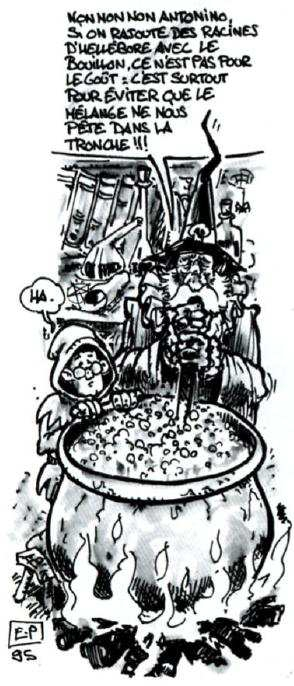
\includegraphics[width=0.30\textwidth]{img/marmiteMaitreApprenti.jpg}

\texttt{<< Inventer >> les composants}

Si on trouve un livre de magie herm{\'e}tique qui contient la liste des composants n{\'e}cessaires {\`a} un sort, il suffit de suivre la recette. Pour ce faire, il faut avoir le talent Alchimie. Deux cas se pr{\'e}sentent.~\\
\begin{itemize}
	\item[\textbf{A)}] On a le niveau de magie requis pour lancer le sort (on poss{\`e}de l'Energie correspondante). Il suffit alors de r{\'e}ussir un test Esprit \imgESPRI + D{\'e}sir \imgDESIR + M{\'e}canique \imgMECAN + Alchimie -- Niveau du sort.
	\item[\textbf{B)}] On veut lancer un sort d'un niveau sup{\'e}rieur de 1 au sien. Il faut alors que le niveau d'Alchimie soit sup{\'e}rieur ou {\'e}gal au niveau du sort que l'on veut atteindre. Par exemple, pour inventer des composants capables de lancer un sort de niveau 2 alors que l'on est au niveau 1, il faut avoir le talent Alchimie {\`a} +2. Le test sera alors Esprit \imgESPRI + D{\'e}sir \imgDESIR + M{\'e}canique \imgMECAN + Alchimie -4.
\end{itemize}

\texttt{Variation des composants}

Le sort de Force de g{\'e}ant que vous avez appris n{\'e}cessite du sang de g{\'e}ant pour {\^e}tre lanc{\'e} plus facilement. Or vous venez d'occire un {\'e}l{\'e}phant (pauvre b{\^e}te). Vous vous dites qu'apr{\`e}s tout, le sang d'{\'e}l{\'e}phant fera aussi bien l'affaire.~\\
~\\~\\
La d{\'e}cision revient au meneur de jeu, qui doit autoriser ce genre de substitutions tant qu'elles restent logiques. Mais le personnage lui ne conna{\^i}tra la r{\'e}ponse {\`a} cette question qu'en r{\'e}ussissant un test Esprit \imgESPRI + Perception \imgPERCE + M{\'e}canique \imgMECAN + Alchimie -2.~\\

\texttt{P{\'e}rennit{\'e} des composants}

Le fait de lancer un sort ne fait pas dispara{\^i}tre les composants du sort.~\\

Ainsi, l'usage d'une loupe pour am{\'e}liorer les chances de r{\'e}ussite d'un sort de Suivre les traces n'envoie pas la loupe dans les limbes {\`a} la fin du sort.~\\

Par contre, il existe de tr{\`e}s nombreux sorts pour lesquels le composant soit {\^e}tre utilis{\'e} au consomm{\'e} (boire un liquide, br{\^u}ler une bougie, d{\'e}chirer un tissu ...), mais cela est fait de fa\c{c}on m{\'e}canique et non pas magique.~\\

\textbf{\textit{Ma{\^i}trise d'arme et parade}}

Dans SimulaceS, que vous sachiez bien vous battre ou pas, si votre adversaire arrive {\`a} passer votre d{\'e}fense, vous subissez l'int{\'e}gralit{\'e} des d{\'e}g{\^a}ts de son arme, comme si vous ne vous {\'e}tiez pas d{\'e}fendu. Cette m{\'e}thode a l'avantage de la rapidit{\'e}, mais semble un peu << injuste >> {\`a} l'encontre des v{\'e}t{\'e}rans du combat qui devraient avoir un peu plus de chance de survivre (avec 5 ou 6 points de vie, la mort n'est jamais tr{\`e}s loin). La r{\`e}gle est donc la suivante : Quand un personnage a un talent d'arme {\`a} +1 ou plus (ou qu'il a le m{\'e}tier Guerrier), sa marge de r{\'e}ussite est retir{\'e}e de la marge de r{\'e}ussite de son adversaire, m{\^e}me si celui-ci a r{\'e}ussi {\`a} le blesser.~\\ 

Exemple : Albrus (+1 en Ep{\'e}e longue) affronte Bertrand (+1 en Hache {\`a} une main). Albrus fait son test de combat et obtient une marge de r{\'e}ussite (MR) de 4. Bertrand fait mieux et a une MR de 5. Dans les r{\`e}gles normales, Bertrand lance 2d6 qu'il ajoute {\`a} sa MR. Disons 7, ce qui donne $7+5=12$ ; face {\`a} une hache, Albrus perd 4PV et 1PS. Avec la nouvelle r{\`e}gle, la MR de Bertrand est diminu{\'e}e de 4 points (MR d'Albrus), ce qui donne au final $12-4=8$, soit une perte de << seulement >> 2PV et 1PS.~\\

Gr{\^a}ce {\`a} son talent de combat, Albrus a mieux su se battre qu'un d{\'e}butant et a {\'e}vit{\'e} une partie du coup. En ce qui concerne les PMJ, accordez cette possibilit{\'e} {\`a} tous les guerriers confirm{\'e}s (qu'il soient Faibles, Moyens ou forts n'a pas d'importance).~\\

Accordez aussi, si vous le d{\'e}sirez, ce talent aux monstres les plus << combatifs >>.~\\

Cette r{\`e}gle permet d'utiliser enfin efficacement le bouclier en parade (SimulacreS p.38). une r{\`e}gle qui, il faut le reconna{\^i}tre, n'est pas tr{\`e}s int{\'e}ressante alors {\`a} appliquer.~\\

%% \clearpage

\colorbox{lightgrey}{ %
\begin{minipage}[ht]{0.30\textwidth}
% \textcolor{magenta}{ }
\textbf{\textit{Rectificatif et pr{\'e}cisions aux r{\`e}gles de SimulacreS}}~\\

\texttt{Puissance et combat}~\\

Dans l'usage optionnel des Energies, rajouter 1 point en Puissance \imgPUISS ne peut {\^e}tre fait que de fa\c{c}on ponctuelle dans un combat, et non de fa\c{c}on continue. Ce qui veut dire qu'utiliser 1EP pour augmenter sa MR ne marche que pour la passe d'armes en cours et non pour les suivantes.~\\

Si vous d{\'e}sirez utiliser la Puissance \imgPUISS pour toute la dur{\'e}e du combat en d{\'e}pensant 1EP, cela se traduirait plut{\^o}t par un bonus de 1 d{\'e} au lancer des d{\'e}g{\^a}ts, c'est-{\`a}-dire pour augmenter les d{\'e}g{\^a}ts en cas de toucher, mais pas pour augmenter les chances de porter un coup.~\\

\texttt{Temps et magie}~\\

Quand un sort demande un temps de concentration sup{\'e}rieur ou {\'e}gal {\`a} une heure dans sa version de base, on doit toujours payer la d{\'e}pense d'Energie avec de l'Equilibre Psychique (EP) et pas avec des points de Souffle (PS), m{\^e}me si on a diminu{\'e} le temps avec de la Rapidit{\'e} \imgRAPID.~\\

Les sorts demandant une longue concentration sont toujours tr{\`e}s {\'e}prouvants psychiquement.~\\ 

Exemple : Un sort d'invocation de Faerie demande un temps de concentration d'une heure. Si on d{\'e}cide de faire passer le temps de concentration {\`a} 30mn en d{\'e}pensant un point de Rapidit{\'e} \imgRAPID, on peut utiliser 1PS pour la Rapidit{\'e} \imgRAPID ; mais le sort lui-m{\^e}me (du niveau 1) n{\'e}cessite toujours de d{\'e}penser 1EP et non 1PS (m{\^e}me si le temps final est pass{\'e} sous la barre d'une heure).~\\

Au contraire, un sort dont le temps de concentration a {\'e}t{\'e} allong{\'e} (en utilisant des composantes gestuelles et verbales par exemple) au-del{\`a} d'une heure n{\'e}cessite bien de d{\'e}penser des EP et plus des PS.~\\
\end{minipage} } %

} % end footnotesize
\end{multicols*} 

\clearpage

\section{Le laboratoire de Ma{\^i}tre Rikeirg}

\texttt{\scriptsize{(Source : Casus Belli n 80 texte : Pierre ROSENTHAL, illustration : DGx)}}

\begin{multicols}{3}
\footnotesize{

\textbf{Le feu tomb{\'e} du ciel}~\\
Les personnages de vos joueurs passent, au cours d'un de leurs p{\'e}riples, dans une petite bourgade {\`a} flanc de montagne.~\\

Dans la nuit, un trait de feu d{\'e}chire le ciel, suivi d'un bruit gigantesque. C'est une m{\'e}t{\'e}orite qui est venue s'{\'e}craser sur le roc, {\`a} quelques centaines de m{\`e}tres d'altitude. Au petit matin, les villageois montent une exp{\'e}dition pour aller voir de quoi il retourne. Les vieux indiquent que l'objet c{\'e}leste s'est {\'e}cras{\'e} au lieu-dit Les Guerriers de Pierre. Il s'agit d'un plateau sur lequel tr{\^o}ne cinq statues d'aventuriers.~\\

Quand l'exp{\'e}dition arrive sur place, les statues sont pulv{\'e}ris{\'e}es, et derri{\`e}re elles la montagne est ouverte, une fissure large comme deux hommes semble s'enfoncer au coeur du roc.~\\

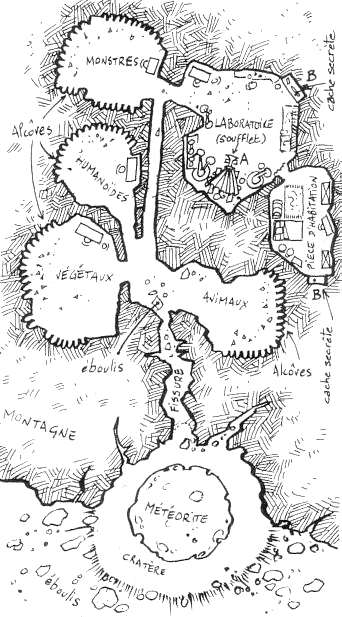
\includegraphics[width=0.30\textwidth]{img/planLaboratoireMaitreRikeirg.jpg}

\textbf{L'histoire}~\\

Il y a quelques si{\`e}cles vivait l{\`a} Rikeirg, un magicien tr{\`e}s puissant pratiquant la magie de la Terre. Passionn{\'e} de biologie, zoologie et botanique, il d{\'e}cida de cr{\'e}er dans son laboratoire, au coeur de la montagne, une gigantesque r{\'e}serve des diverses esp{\`e}ces vivantes. Pour cela, il utilisa l'un de ses plus puissants sortil{\`e}ges : Pulv{\'e}risation (r{\'e}versible), qui permet de transformer un {\^e}tre vivant en poussi{\`e}re. Son laboratoire {\'e}tait jusqu'alors inaccessible puisque Rikeirg le rejoignait en passant directement {\`a} travers la pierre. Le magicien est aujourd'hui mort depuis longtemps, et son laboratoire contient quantit{\'e}s de fioles remplies de poussi{\`e}re, d'{\^e}tres vivants n'attendant plus que leur r{\'e}surrection.~\\

\textbf{Les cavernes}~\\

Rikeirg a construit son laboratoire dans un r{\'e}seau de cavernes. Les pi{\`e}ces principales sont : le laboratoire de magie proprement dit, la pi{\`e}ce d'habitation, la salle des {\^e}tres v{\'e}g{\'e}taux, la salle des animaux, la salle des monstres, la salle des humano{\"i}des. A vous de d{\'e}velopper ce r{\'e}seau de cavernes en fonction de l'importance que vous d{\'e}sirez donner {\`a} l'aventure. De plus, au moment o{\`u} la m{\'e}t{\'e}orite a ouvert la montagne, elle a d{\'e}clench{\'e} un sortil{\`e}ge de protection. Il consiste en l'invocation d'un {\'e}l{\'e}mental de terre charg{\'e} de garder le laboratoire pour les trois ann{\'e}es {\`a} venir, sauf si Rikeirg revient prendre possession de son bien.~\\

L'{\'e}l{\'e}mental reconna{\^i}tra le magicien {\`a} sa bague. Suivant le niveau des personnages-joueurs, vous pouvez d{\'e}cider de ne pas utiliser l'{\'e}l{\'e}mental, qui est une cr{\'e}ature particuli{\`e}rement puissante.~\\

De plus il y a tr{\`e}s peu d'air dans les cavernes, les torches s'{\'e}teignent tr{\`e}s vite, les personnages qui ne r{\'e}ussissent pas un test Corps \imgCORPS + R{\'e}sistance \imgRESIS + Humain \imgHUMAI + 3 toutes les 15 minutes se mettent {\`a} suffoquer (et perdent 1 PS).~\\

\textbf{Le laboratoire}~\\

Il contient de nombreux alambics et fioles, recouverts de poussi{\`e}re. Les personnages qui poss{\`e}dent les talents Alchimie ou Art magique reconnaissent un laboratoire magique sp{\'e}cialis{\'e} dans la cr{\'e}ation d'objets magiques. Dans une boite en acier, un livre en cuir aux pages extr{\^e}mement s{\`e}ches et fragiles contient quelques renseignements. Il explique comment Rikeirg a d{\'e}cid{\'e} de cr{\'e}er cette "Arche de No{\'e}" en poussi{\`e}re, mais il ne donne pas la recette magique pour reproduire son sortil{\`e}ge. Un magicien peut juste comprendre qu'il s'agit d'un sort tr{\`e}s puissant (donc de niveau 3), et que la cr{\'e}ature est r{\'e}duite {\`a} un poids de poussi{\`e}re {\'e}gal au centi{\`e}me de son poids normal. Rikeirg indique par contre qu'il a cr{\'e}{\'e} une baguette qui permet de lancer le sort inverse (et donc de redonner vie {\`a} la poussi{\`e}re), et que certains flacons ont {\'e}t{\'e} enchant{\'e}s de fa\c{c}on {\`a} ce que la cr{\'e}ature revienne {\`a} la vie d{\`e}s le bouchon est {\^o}t{\'e}. Il indique aussi qu'un sortil{\`e}ge d'annulation de la magie peut avoir le m{\^e}me effet (avec une grosse difficult{\'e}).~\\

Dans un coin de la pi{\`e}ce une machinerie gigantesque fait penser {\`a} un immense soufflet. C'est un g{\'e}n{\'e}rateur magique d'air. Pour le faire fonctionner, il faut se concentrer dessus et r{\'e}ussir un test Esprit \imgESPRI + Action \imgACTIO + N{\'e}ant \imgNEANT + Art magique, et d{\'e}penser 1 PS ou 1 EP. Si on d{\'e}pense 1 PS il fonctionne pendant une heure, si c'est 1 EP, il fonctionne pendant une semaine. Il g{\'e}n{\`e}re en deux heures suffisamment d'air pour remplir le r{\'e}seau de cavernes.~\\

Si un personnage fouille le laboratoire et r{\'e}ussit un test Corps \imgCORPS + Perception \imgPERCE + Min{\'e}ral \imgMINER + Ma\c{c}onnerie, il trouve une cache secr{\`e}te. L'int{\'e}rieur contient une baguette en marbre vert et une dague. La baguette est un objet {\`a} focus qui contient 3PM au maximum (et qui est {\`a} son maximum pour le moment). Elle ne contient qu'un seul sortil{\`e}ge, celui qui permet, en touchant la poussi{\`e}re magique, de recr{\'e}er l'{\^e}tre d'origine. La baguette n'est pas pi{\'e}g{\'e}e, mais si le magicien qui l'utilise ne met pas au moment du lancer 1 PS ou 1 EP de lui-m{\^e}me, ce sont les 3 points de l'objet qui sont utilis{\'e}s en totalit{\'e} et celui-ci deviendra alors inutile (puisqu'{\`a} 0 PM). Alors que s'il reste au moins 1PM dans l'objet, on peut toujours le recharger (voir les r{\`e}gles dans \textbf{SimulacreS} ou \textbf{SangDragon}). La dague fait des d{\'e}g{\^a}ts normaux mais elle est enchant{\'e}e, cela veut dire qu'elle peut infliger des d{\'e}g{\^a}ts normaux {\`a} des {\^e}tres magiques.~\\

\textbf{La pi{\`e}ce d'habitation}~\\

En dehors d'une couche et d'une armoire qui contient quelques v{\^e}tements presque r{\'e}duits en poussi{\`e}re, on peut remarquer :
\setlength\parindent{20pt}
\begin{itemize}
		\item Les restes d'un squelette sur le lit. Rikeirg, mort vieux et malade, d'asphyxie.
		\item Un des murs abrite une cache secr{\`e}te qui contient une bague en obsidienne, avec un R en monogramme. C'est la bague de Rikeirg, et si l'{\'e}l{\'e}mental est encore pr{\'e}sent, il ob{\'e}ira {\`a} celui qui la porte.
\end{itemize}~\\
\setlength\parindent{0pt}

\begin{center}
	
\includegraphics[width=0.25\textwidth]{../../../../../imgGraphics/artsDecos/flowersL2R.png}
\end{center}

\clearpage

\textbf{Les salles}~\\

Soigneusement rang{\'e}es dans des alc{\^o}ves de pierre, il y a des centaines de fioles de verre remplies de poussi{\`e}re, plus ou moins grosses. Malheureusement, le choc de la m{\'e}t{\'e}orite en a pr{\'e}cipit{\'e} plus de la moiti{\'e} {\`a} terre o{\`u} elles se sont bris{\'e}es et m{\'e}lang{\'e}es. Sous chaque fiole dans son alc{\^o}ve, sont grav{\'e}es quelques runes qui en indiquent le contenu. C'est une vieille {\'e}criture, presque oubli{\'e}e, mais relativement proche de l'{\'e}criture naine. Toutes les fioles irradient la magie (si on la d{\'e}tecte) en raison de la poussi{\`e}re. Elles sont toutes ferm{\'e}es par un bouchon de cristal et scell{\'e}es par un m{\'e}lange de gel et de graisse. Si on regarde de pr{\`e}s les bouchons (Corps \imgCORPS + Perception \imgPERCE + Min{\'e}ral \imgMINER -- 2), on remarque que certains pr{\'e}sentent de l{\'e}g{\`e}res runes incrust{\'e}es.~\\

Ce sont des fioles qui, {\`a} l'ouverture, d{\'e}clenchent instantan{\'e}ment le sort de retour {\`a} la vie de leur contenu. Ce sortil{\`e}ge ne fonctionne qu'une seule fois.~\\
Si on utilise le sortil{\`e}ge de la baguette sur la poussi{\`e}re du sol (m{\'e}lange des fioles bris{\'e}es), voici ce qui risque de se passer :
\begin{tabular}[ht]{ p{0.05\textwidth} p{0.25\textwidth} }
	\rowcolor{white}	\textbf{2d6} 	&	\textbf{R{\'e}sultat}					\\
	\rowcolor{gray}		2				&	Une cr{\'e}ature rare se recompose		\\
	\rowcolor{white}	3				&	Une cr{\'e}ature commune se recompose	\\
	\rowcolor{gray}		4-10			&	Rien									\\
	\rowcolor{white}	11				&	Une chim{\`e}re monstrueuse (m{\'e}lange de plusieurs esp{\`e}ces) se compose, agressive.		\\
	\rowcolor{gray}		12				&	Explosion. Toutes les personnes pr{\'e}sentes subissent [d+2] PV et [e+4] PS de d{\'e}g{\^a}ts.	\\
\end{tabular}~\\~\\

\textbf{La salle v{\'e}g{\'e}tale}~\\ 

Il y a environ trois cents fioles dans cette r{\'e}serve, dont une centaine est encore intacte. Aucune fiole n'est enchant{\'e}e pour une recomposition automatique. Parmi les plantes les plus exotiques on trouve : un arbre {\`a} dryade (qui est pr{\`e}s "d'accoucher" d'un de ces {\^e}tres mythiques), un lierre carnivore (qui envoie des spores somnif{\`e}res), un Latexia Salvateur (on coupe l{\'e}g{\`e}rement le tronc de l'arbre pour laisser le latex s'{\'e}chapper, et on recouvre avec une blessure, ou un membre mutil{\'e}. Il faut que la s{\`e}ve soit toujours en contact avec l'int{\'e}rieur de l'arbre. Les blessures se gu{\'e}rissent alors en 24 heures et les membres se r{\'e}parent en une semaine).~\\

\textbf{La salle animale}~\\

Il reste cinquante fioles intactes sur les cent quatre-vingt-six qu'il y avait. Quelques-unes recomposent les animaux d{\`e}s qu'on ouvre le bouchon : ce sont l'aigle, le chien de guerre, le cheval de Rikeirg, mais aussi un couple de vaches, de moutons, de lapins, de poules, de cochons, d'{\'e}l{\'e}phants.~\\

On trouve par ailleurs quelques animaux exotiques : girafe, cobra cracheur, lion, dauphin, grizzly...~\\

\textbf{La salle humano{\"i}de}~\\

Seules cinquante fioles sont intactes sur les cent originelles. Aucune fiole n'est enchant{\'e}e pour une recomposition automatique. Rikeirg avait pour habitude de pulv{\'e}riser des condamn{\'e}s {\`a} mort, des brigands, etc. Autant dire que les ramener {\`a} la vie risque de poser des probl{\`e}mes.~\\

On trouve d'ailleurs dans les fioles les poussi{\`e}res de Maevilder, un tr{\`e}s puissant n{\'e}cromancien, ennemi jur{\'e} de Rikeirg, et Laena, une elfe assassin d'une fascinante beaut{\'e} compagne du n{\'e}cromancien.~\\

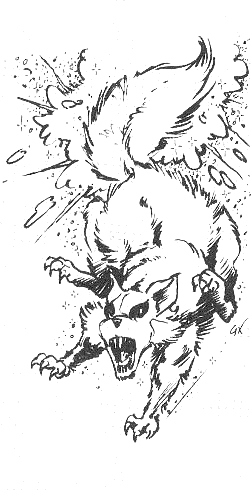
\includegraphics[width=0.30\textwidth]{img/verteneRikeirg.jpg}

\textbf{La salle monstrueuse}~\\

Environ quarante fioles subsistent sur les deux cents pr{\'e}sentes. Evidemment, aucun mort-vivant n'est dans le lot (le sortil{\`e}ge ne fonctionne pas sur eux) ni aucune cr{\'e}ature infernale ou {\'e}l{\'e}mentaire. Parmi les fioles qui se recomposent automatiquement il y a : un dragon rouge adulte (et en col{\`e}re), une m{\'e}duse (une femme hideuse aux cheveux serpentins, dont le regard p{\'e}trifie qui la fixe), une amibe g{\'e}ante (qui mange le bois). Parmi les autres monstres : une vert{\`e}ne (sorte d'{\'e}cureuil qui d{\'e}tecte la magie) ; un sicriard (hamster crieur) dont la fiole porte en langage commun: danger ; plus autant d'autres que vous le d{\'e}sirerez. ~\\

% \vfill

\colorbox{lightgrey}{ %
\begin{minipage}[ht]{0.30\textwidth}
% \textcolor{magenta}{ }
\textbf{Annulation de la magie}~\\

Sortil{\`e}ge de magie Herm{\'e}tique, Niv. 2~\\
Difficult{\'e} d'apprentissage : -4~\\
Difficult{\'e} de lancer : 0~\\
Dur{\'e}e d'incantation : 2 heures~\\
Dur{\'e}e du sort : instantan{\'e}e~\\
Port{\'e}e : contact~\\
Effet : ce sort est tr{\`e}s puissant puisqu'il annule toute magie d'un lieu, objet ou cr{\'e}ature. Il vide les focus de tous leurs points de magie. Par contre si la difficult{\'e} de lancer du sortil{\`e}ge est de 0, celui-ci ne r{\'e}ussit que si la MR est sup{\'e}rieure {\`a} celle du magicien qui avait lanc{\'e} le sortil{\`e}ge. Si rien n'est pr{\'e}cis{\'e}, on supposera qu'elle {\'e}tait de 3. De plus, ce sortil{\`e}ge est risqu{\'e} {\`a} lancer. Si on y arrive pas ({\'e}chec du lancer et pas de l'effet du sortil{\`e}ge) on perd [c] EP, [e] PS et [a] PV. En ce qui concerne les cr{\'e}atures des fioles, Rikeirg a r{\'e}ussi son sortil{\`e}ge {\`a} chaque fois avec un score allant de 3 {\`a} 8 (1D6+2) (et exceptionnellement une ou deux fois {\`a} 15).~\\

\textbf{Amibe g{\'e}ante}~\\

Test de combat : 5~\\
Test de perception : 4~\\
Points de vie : 3, Points de souffle : -- ~\\
D{\'e}g{\^a}ts : [a] PV, Armure : 0/0/8~\\
L'amibe fait environ 1m de long et de large, sur quelques centim{\`e}tres d'{\'e}paisseur. Elle mange et ronge le bois (une porte normale en une heure). Ses d{\'e}g{\^a}ts proviennent du l{\'e}ger acide qu'elle distille.~\\

\textbf{Vert{\`e}ne}~\\
Test de combat : 6~\\
Test de perception : 8~\\
R{\'e}sistance {\`a} la magie : 10~\\
Points de vie : 2, Points de souffle : 2~\\
Points d'Energie : 2, Rapidit{\'e} : 2~\\
D{\'e}g{\^a}ts : [b] PV, Armure : 0/0/0~\\
La vert{\`e}ne est un esp{\`e}ce d'{\'e}cureuil qui vit dans un terrier. Elle d{\'e}tecte la magie et collectionne les objets magiques de petite taille. Elle a constamment besoin de manger, m{\^e}me apprivois{\'e}e. Si on la met en col{\`e}re, elle mord. En plus des d{\'e}g{\^a}ts, une morsure de vert{\`e}ne occasion 1 point de Malaise (qui dure 24 heures). Et la peau du bless{\'e} devient d'un vert maladif (durant 48 heures).~\\

\textbf{Sicriard}~\\

Pas de caract{\'e}ristique pour ce hamster qui est trop faible pour faire quoi que ce soit. Il vit environ deux ans. D{\`e}s que le sicriard se sent en danger, il pousse un cri per\c{c}ant qui pulv{\'e}rise tous les mat{\'e}riaux en verre {\`a} moins de cinq m{\`e}tres de lui. La c{\'e}ramique et la terre cuite sont parfois un peu {\'e}branl{\'e}es.~\\
\end{minipage} } %

} % end footnotesize
\end{multicols} 

\clearpage

\section{Le guide intergalactique du barbare scientifique}

\texttt{\scriptsize{(Source : \textbf{Casus Belli} n 75 / \textbf{Petit Capharna{\"u}m} n 12, texte : \textbf{Pierre ROSENTHAL/Pierre Nicolas LAPOINTE)} } }~\\ 

\textbf{\textit{\small C'est la derni{\`e}re fois que parait cette formule du petit capharna{\"u}m en une page. De m{\^e}me que la Gazette galactique. En effet, une page r{\'e}guli{\`e}re c'est bien, mais une page c'est trop peu pour d{\'e}vilopper une id{\'e}e d'univers, des r{\`e}gles,etc. chacune de ces r{\'e}publiques aura donc droit {\`a} deux pages, mais un num{\'e}ro sur deux en alternance. C'est M{\'e}ga III qui inaugurera la nouvelle formule. {\`A} dans deux num{\'e}ros donc. }}~\\

\begin{multicols}{3}
\small{

Pierre-Nicolas Lapointe est un jeune auteur talentueux, {\`a} qui on doit notamment les jeux \emph{Sombre Cauchemar} (jeu horrifico-rigolo {\'e}dit{\'e} {\`a} compte d'auteur), \emph{Enfer \& Damnation} (dans \emph{Jeux et Strat{\'e}gie}) et une participation aux bestioles bizarres d'Alieno{\"i}ds. Il nous a envoy{\'e} ce texte, qui peut tr{\`e}s bien servir dans n'importe quel jeu d'anticipation o{\`u} on ne se prend pas trop au s{\'e}rieux.~\\

\textbf{Le Guide intergalactique du barbare scientifique}~\\

Tout le monde peut facilement imaginer {\`a} quoi ressemble un ch{\^a}teau fort. Cela fait partie de notre patrimoine culturel.~\\

En mati{\`e}re de science-fiction, le d{\'e}cor est beaucoup plus d{\'e}licat {\`a} imaginer. Comment faire pour emballer ses joueurs et leur faire croire qu'ils {\'e}voluent vraiment dans un univers futuriste, un des moyens les plus simples est d'employer naturellement scientifique incompr{\'e}hensible. Cette gymnastique n'est pas {\`a} la port{\'e}e de tous les meneurs de jeu, c'est pourquoi je vous propose le \emph{Guide intergalactique du barbare scientifique}, {\`a} employer sans mod{\'e}ration tout au long de la partie.~\\

\texttt{Mode d'emploi}~\\
Pour former un nouveau barbarisme scientifique, il suffit de piocher al{\'e}atoirement un mot dans chaque table, en partant de la table 1 {\`a} la table 4. pour varier les plaisirs, vous trouverez facilement des moyens d'interchanger et de doubles les tables : la suite objet-pr{\'e}fixe-fonctionnature-pr{\'e}fixe-fonction fait des merveilles ! Exemple : {\'E}voquez n{\'e}gligemment l'{\'e}pisode o{\`u} vous avez sauv{\'e} vos compagnons en r{\'e}parant le vibrom{\`e}tre hydro-magn{\'e}tique {\`a} effet gyrom{\'e}trique ...~\\

La table 5/ Position est particuli{\`e}rement int{\'e}ressante quand il s'agit de d{\'e}signer une panne {\`a} bord d'un vaisseau spatial. {\`A} propos de pannes, vous pouvez aussi vous r{\'e}f{\'e}rer {\`a} la liste de quelques verbes utiles dans la panique d'un combat spatial. Malgr{\'e} tous mes efforts, je suis s{\^u}r d'avoir oubli{\'e} plein de mots que vous aurez la joie de rajouter aux tables.~\\

\textbf{Et pour quelques suppl{\'e}ments de plus}~\\

J'ai re\c{c}u plusieurs suppl{\'e}ments SimulacreS durant ces deux derniers mois. Ils ont pour noms \textbf{Le Baron de Munchausen}, \textbf{CyberCommando} et \textbf{Justice for All}. Vous trouverez une rapide pr{\'e}sentation de ces univers dans les pages de Pr{\'e}visions m{\'e}t{\'e}oludiques (Nouvelles du Front). Merci {\'e}galement {\`a} ceux qui m'ont {\'e}crit au sujet d'une deuxi{\`e}me {\'e}dition de SimulacreS.~\\

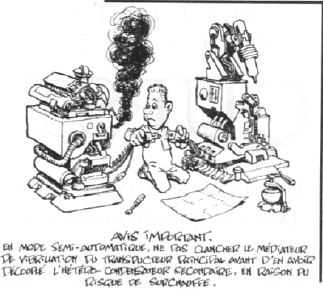
\includegraphics[width=0.30\textwidth]{img/barbarismeScientifique.jpg}

} % end small
\end{multicols}

\clearpage

\begin{table}[ht]
	\begin{multicols}{5}
	\small{
	
\textbf{Table 1 -- Objet}~\\
1	Alternateur~\\
2	Batterie~\\
3	Booster~\\
4	Bouclier~\\
5	Cabine~\\
6	Cale~\\
7	Carburateur~\\
8	Champs~\\
9	Circuits~\\
10	Comburant~\\
11	Compteur~\\
12	Computer~\\
13	Condensateur~\\
14	Coupleur~\\
15	Cyclotron~\\
16	D{\'e}flecteur~\\
17	Driver~\\
18	Essuie-glace~\\
19	Extincteur~\\
20	Fus{\'e}e~\\
21	G{\'e}n{\'e}rateur~\\
22	Injection~\\
23	Laser~\\
24	Levier~\\
25	Liquide~\\
26	Ordinateur~\\
27	Oscillateur~\\
28	Pression~\\
29	Processus~\\
30	Pulseur~\\
31	Radio~\\
32	Senseurs~\\
33	Stabilisateur~\\
34	Transducteur~\\
35	Ventilo~\\
36	Vibrom{\`e}tre~\\
37	Vobulateur~\\

\columnbreak

\textbf{Table 2 -- Nature ({\`a}...)}~\\
1	Avancement~\\
2	Combustion~\\
3	Condensation~\\
4	Conditionnement~\\
5	Effet~\\
6	Energie~\\
7	Frottement~\\
8	Glissement~\\
9	Impact~\\
10	M{\'e}diation~\\
11	M{\'e}moire~\\
12	Ascillation~\\
13	Positionnement~\\
14	Pression~\\
15	Propension~\\
16	Pulsion~\\
17	Rayonnement~\\
18	R{\'e}action~\\
19	Refroidissement~\\
20	Retardement~\\
21	Stabilisation~\\
22	Tension~\\
23	Turbulence~\\
24	Vibration~\\

\rule{0.15\textwidth}{0.05cm}~\\

\textbf{Verbes de pannes}~\\
1	A des rat{\'e}s~\\
2	A rip{\'e}~\\
3	Bourjouffle~\\
4	D{\'e}lire~\\
5	D{\'e}rape~\\
6	Disjoncte~\\
7	Est {\`a} plat~\\

\columnbreak

\textbf{Table 3 -- Pr{\'e}fixe}~\\
1	A{\'e}ro~\\
2	Astro~\\
3	Bi~\\
4	Bio~\\
5	Carbo~\\
6	Cryo~\\
7	Gyro~\\
8	H{\'e}t{\'e}ro~\\
9	Homo~\\
10	Hydro~\\
11	Hyper~\\
12	Inter~\\
13	Interf{\'e}ro~\\
14	Magn{\'e}to~\\
15	M{\'e}ga~\\
16	M{\'e}ta~\\
17	Philo~\\
18	Prolo~\\
19	R{\'e}tro~\\
20	Roto~\\
21	Servo~\\
22	Super~\\
23	Thermo~\\
24	Turbo~\\
25	Vibro~\\

\rule{0.15\textwidth}{0.05cm}~\\

8	Est dans le rouge~\\
9	Est K.O.~\\
10	Est mort~\\
11	Est naze~\\
12	Flanche~\\
13	Fuit~\\
14	Grille {\`a} fond~\\
15	Ne r{\'e}pond plus~\\

\columnbreak

\textbf{Table 4 -- Fonction}~\\
1	Actif~\\
2	Athermogile~\\
3	Atomique~\\
4	Automatique~\\
5	Biog{\'e}rique~\\
6	Dynamique~\\
7	Electronique~\\
8	Energique~\\
9	H{\'e}t{\'e}rodyne~\\
10	Ionique~\\
11	Magn{\'e}tique~\\
12	Manuel~\\
13	M{\'e}trique~\\
14	Mol{\'e}culaire~\\
15	Neuronal~\\
16	Nucl{\'e}aire~\\
17	Optique~\\
18	Posotronique~\\
19	Puls{\'e}~\\
20	R{\'e}gul{\'e}~\\
21	Retard{\'e}~\\
22	Sinuso{\"i}dal~\\
23	Stabilis{\'e}~\\
24	Statique~\\
25	Triangulaire~\\

\rule{0.15\textwidth}{0.05cm}~\\


16	S'enflamme~\\
17	Se d{\'e}visse~\\
18	Se dilate~\\
19	Se disloque~\\
20	Tourne dans le vide~\\
~\\
~\\
~\\

\columnbreak

\textbf{Table 5 -- Position}~\\
1	Arri{\`e}re~\\
2	Avant~\\
3	Central~\\
4	Se secours~\\
5	De soutien~\\
6	Invers{\'e}~\\
7	Lat{\'e}ral~\\
8	Parall{\`e}le~\\
9	Principal~\\
10	Relatif~\\
11	Secondaire~\\

\rule{0.15\textwidth}{0.05cm}~\\

\rule{0.15\textwidth}{0.05cm}~\\

\rule{0.15\textwidth}{0.05cm}~\\
	
	} % end small
	\end{multicols}
	\caption{Pour g{\'e}n{\'e}rer quelques barbarismes scientifiques de bon go{\^u}t...}
\end{table}

% \imgCORPS~\\
% \imgINSTI~\\
% \imgCOEUR~\\
% \imgESPRI~\\

% \imgPERCE~\\
% \imgACTIO~\\
% \imgDESIR~\\
% \imgRESIS~\\

% \imgMINER~\\
% \imgVEGET~\\
% \imgANIMA~\\
% \imgHUMAI~\\
% \imgMECAN~\\
% \imgNEANT~\\

% \imgPUISS~\\
% \imgRAPID~\\
% \imgPRECI~\\

\end{document}
